\subsection{Execution stage}
The execution stage contains the blocks that carry out the calculations, including the ALU, the Forwarding Unit, the PC incrementer and some useful units to manage data flows. Each operation lasts one clock cycle so there are no pipeline stages within the stage but only before and after. In figure \todo{Insert figure} all the blocks and the data path can be seen.\\
The ALU has two inputs which are partly managed by the instruction decoded by the CU and partly by the forwarding unit in case data dependencies are present. In the case of non-hazardous operation, port "A" of the ALU contains data "A" from the register file or the non-incremented PC, while port "B" contains data from port "B" of the register file or the Immediate from the instruction. In this way all instructions can be handled without ever having an overlap in the port request. On the other hand, when data dependencies are present, these data are ignored and bypassed by the forwarding unit's decision in order to insert the correct data. The management of the branch instruction requires the evaluation of equality between two data and is carried out by a separate unit from the ALU as it is busy in calculating the jump address, i.e. the sum between the PC and the displacement present in the Immediate. Some units are analysed in detail in the following subsections.

\subsubsection{ALU}
The Arithmetic Logic Unit is one of the most important blocks in a digital system; in fact the performances of CPUs, $\mu$Controllers and $\mu$Processors, are strictly dependent on the ALU structure. Because of this, the component must be developed according to the applications in which it will be used. For example, in a high-performance computer, the ALU must be designed favouring the speed of the logic and arithmetic components, penalising consumption and the occupied area. Conversely, in low-power applications, the component must be economical and dissipate a low amount of power. In the case of RISC-V, the system has to be fast and latency is expected to be low to allow a high clock frequency.  The ALU can perform these seven logical and arithmetic operations:

\begin{itemize}
	\item Addition
	\item Subtraction
	\item AND
	\item XOR
	\item Comparison
	\item Right shift
	\item Operand Feedforward
\end{itemize}
\noindent
The first six instructions perform operations between two numbers, the last one directly outputs the second input of the ALU, but they all work with std\_logic inputs. In addition, the control unit of the ALU drives it with four bits and in case of wrong input control, the component gives zeros as output.

\subsubsection{Carry Select Adder}
The structure of the adder will be analysed in the following in order to reduce its latency. The purpose is to analyse the costs, latency and fanout at some critical nodes. The Carry Select Adder has been developed from the basic cell of the Full Adder, shown in the \autoref{fig:full_adder}

\begin{figure}[htbp]
	\centering
	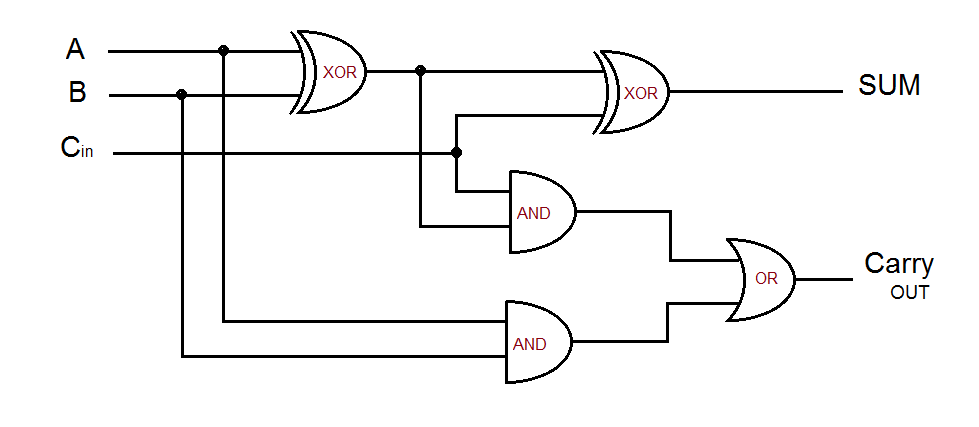
\includegraphics[width=0.5\textwidth]{sec2/images/full_adder.png}
	\caption{Full adder, logic gates schematic}
	\label{fig:full_adder}
\end{figure}
\noindent
This simple block was used to create a not common and not uniform adder structure. In general the adder structure is composed by elementary FA, that are grouped as a power of two: two, four, eight and so on. The implementation was done with six full adders and two full adder at the beginning. The main carry select adder block is showed in \autoref{fig:carry_sel}.

\begin{figure}[htbp]
	\centering
	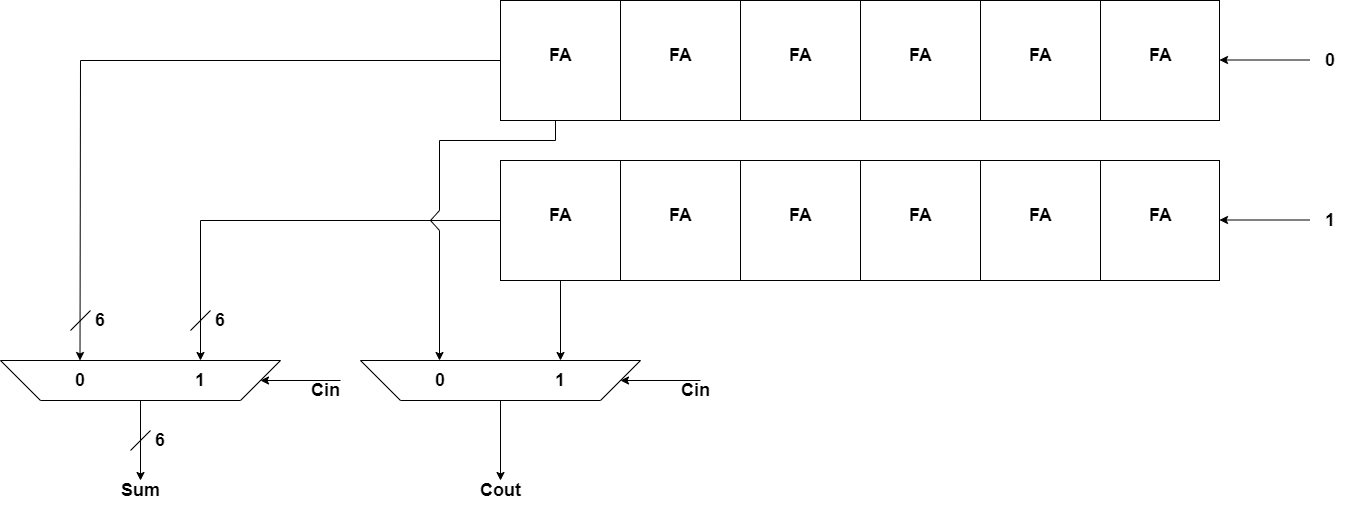
\includegraphics[width=0.7\textwidth]{sec2/images/C_sel_A.png}
	\caption{Carry Select Adder main block}
	\label{fig:carry_sel}
\end{figure}
\noindent
The reason for this choice is the masking of the latency of the first multiplexer, in fact the low latency of the two full adders at the start allows the first multiplexer to be switched before the first main block has even finished calculating. In this way, the latency is characterised by a weaker dependence on the delay of the multiplexer. Considering a total number of five main blocks plus two full adders, the total delay is:
\begin{equation}
	T_{DELAY} = (\frac{N-2}{6} - 1)T_{MUX} + 6T_{FA}
\end{equation}
Where N is the total number of bits.
If compared with a carry save adder with a main block of eight full adders, the total multiplexer delay is the same but there is an advantage with respect to the full adder delay. Furthermore, if the used structure is compared with one based on group of four full adders, the advantage will be observed by looking the total multiplexer delay, that is higher in the second case than the first one.
Now a fanout analysis is going to be done; by looking the \autoref{fig:carry_sel}, there is the necessity to observe the two multiplexer select signal. The equation of these two multiplexer is:
\begin{equation}
	(In_1 \cdot C_{IN}) + (In_2 \cdot \overline{C_{IN}})
\end{equation}

The selector has to drive:
\begin{equation}
	F_{OUT} = 2\cdot 6Wires + 2 \cdot 2Wires = 14Wires
\end{equation}
The selector experiences a very large fanout and it happens in all multiplexers, therefore when the circuit will be synthetized, a driver must be inserted in order to avoid an high load capacitance and an high peak current, in which the first slow the circuit and the second could yield electromigration or burn the logic gates.\\
\noindent The last parameter that must be analysed is the cost, or to be more precise, the total number of components that have to be used in order to develop the adder:
\begin{itemize}
	\item $N_{FA} = 2\cdot N_{BIT} = 64$
	\item $N_{MUX} = 2\cdot \frac{N-2}{6}  = 10$
\end{itemize}
In order to obtain better performances, the cost to be paid is quite high, in fact respect to a simple ripple carry adder, the number of full adder is doubled and in addition there are ten multiplexer, The overall architecture is represented in \autoref{fig:CSA_full}:

\begin{figure}[htbp]
	\centering
	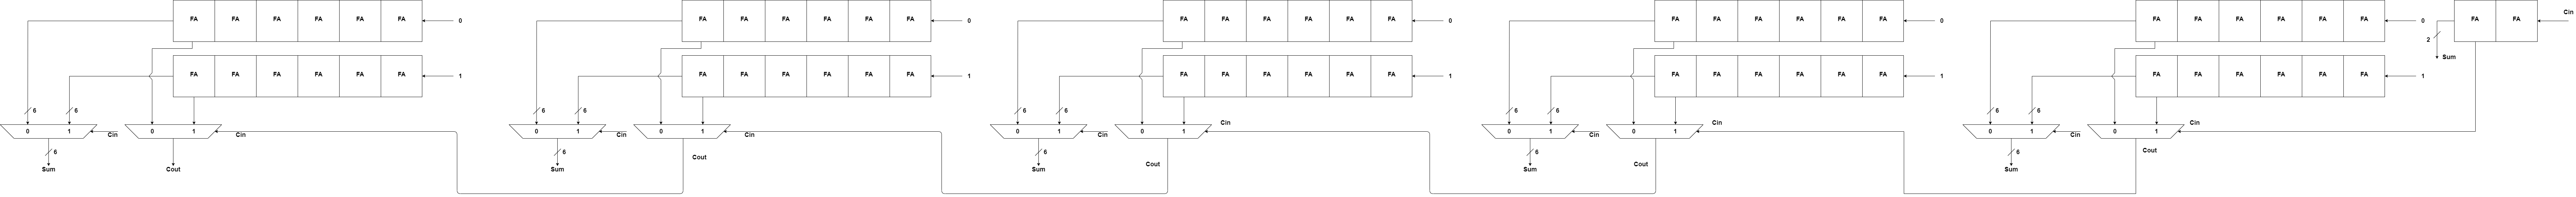
\includegraphics[width=1\textwidth]{sec2/images/CSA_full.png }
	\caption{Carry Select Adder schematic}
	\label{fig:CSA_full}
\end{figure}

\subsubsection{Forwarding Unit}
The forwarding unit is responsible for resolving all data dependencies between the Execute stage and the other pipeline stages. In particular, it looks for situations in which the source register of the current instruction coincides with the destination address of the instruction processed one or two clock cycles earlier.
\begin{figure}[htbp]
	\centering
	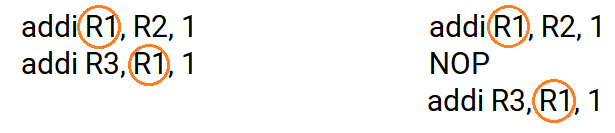
\includegraphics[width=0.5\textwidth]{sec2/images/data_dependency.png}
	\caption{Example of data dependencies solved by the forwarding unit}
	\label{fig:zero_skipping}
\end{figure}
\\In the first case, the data is taken from the output register of the ALU, instead of the register file. In the second case from the memory output register. In this way the data is forwarded without waiting for the correct data to be written in the register file. Each time the forwarding unit starts up, there is a benefit that corresponds to one or two clock cycles. To understand if the bits of the source and destination addresses are valid it is necessary to check that the instructions they refer to use such fields, i.e. if the instruction is of the type \textit{R, I, U, J}.\\
The forwarding unit also handles Store instructions, which write directly to memory by forwarding the data from the ALU output register or the memory output register to the data memory input.\\
Since the branch evaluation is also done on data from the register file, it requires the forwarding of data of both inputs.
